\chapter{Teoría de Aproximaciones: Bases Reducidas y Aprendizaje}


En este capítulo se dará una introducción a las bases reducidas, un método de aproximación fundamental en el modelado de orden reducido \cite{Tiglio:2021ysj}. Este marco posee dos etapas bien diferenciadas; por un lado la parte de entrenamiento que puede ser bastante costosa (\textit{offline}), y después la parte de evaluación, que es mucho más rápida (\textit{online}).

Luego se ampliará con el refinamiento hp \textit{greedy} \cite{Cerino:2022dhr}; una metodología que descompone de forma iterativa el dominio de parámetros para crear bases reducidas locales.

%\section{Aproximación por Proyección}
%Antes de entender las bases reducidas es necesario tener claro como se aproxima un vector o función a un dado espacio.
%Sea $W_n \mathcal{W}_n$ un espacio vectorial n-dimensional y subespacio de un espacio de Hilbert $\mathcal{H}$

\section{Bases Reducidas}

El objetivo de este método es obtener una base que represente un espacio de soluciones de forma aproximada, evitando tener que resolver el problema completo múltiples veces para generar más soluciones. 
En este contexto las soluciones son ondas gravitacionales y resolver el problema consistiría en obtener soluciones a partir de relatividad numérica.

Las bases reducidas son un método de expansión espectral así como la expansión de Fourier o los ponimonios de Jacobi. La diferencia de este método es que los elementos de la base serán soluciones del espacio que se quiere aproximar (no necesariamente funciones trigonométricas o polinomios, como en otros métodos).

Partiendo de un espacio de soluciones $\mathcal{F}:= \{ h_{\lambda} = h_{\lambda}(t) = h(\lambda, t)\}$, donde $h_{\lambda}$ representa una onda gravitacional parametrizada por $\lambda$, que generalmente es multidimensional y puede representar la relación entre las masas de los agujeros negros o los espínes, por ejemplo.

Para construir la base se parte de un conjunto de entrenamiento $\mathcal{T} := \{\lambda_i, h_{\lambda_i}\}_{i=1}^N$, resultado de un muestreo $\mathcal{K} := \{h_{\lambda_i}\}_{i=1}^n$de $\mathcal{F}$, y que contiene la información del conjunto de parámetros $\{\lambda_i\}_{i=1}^n$ utilizado para la construcción de cada función de $\mathcal{K}$. A partir de $\mathcal{T}$ se construye una base $\{e_i\}_{i=1}^n$, generalmente con $n << N$. Luego se puede representar $\mathcal{K}$, e incluso $\mathcal{F}$ con la combinación lineal

\begin{equation}
\label{eq:rb0}
h_{\lambda} (t) \approx \sum_{i=1}^{n} c_{i,\lambda} e_i(t).
\end{equation}

\subsection{Elección de una base óptima}

%Antes de poder representar $\mathcal{F}$ se necesita encontrar una base óptima dado un error de tolerancia $\varepsilon$ y/o un máximo número de elementos en la base $n_{max}$.
La pregunta de que tan bien se puede aproximar el espacio $\mathcal{F}$ lleva a la distancia de Kolmogorov \cite{Pinkus1985nWidthsIA}:

\begin{equation} \label{eq:kolmogorov}
d_n := \min_{\{e_i\}_{i=1}^n} \max_{\lambda \in \Omega} \min_{ c_{i,\lambda} \in \mathbb{C}} || h_{\lambda} - \sum_{i=1}^{n} c_{i,\lambda} e_i(t)||^2.
\end{equation}



Básicamente es una medida del máximo error de representación en un espacio compacto de parámetros $\Omega$, con una base y coeficientes óptimos.
El producto interno $||\cdot||$ está dado por

\[
||h_{\lambda}||^2 :=\int_{t_i}^{t_f}|h_{\lambda}(t)|^2dt
\]
definido a partir del producto interno
\[
\langle h_1, h_2 \rangle  :=\int_{t_i}^{t_f} \overline{h_{1}}(t) h_2 (t)dt
\]

Para entender la notación en $d_n$, analizando los $\min$, $\max$ y $\min$ de derecha a izquierda:

\begin{itemize}
\item $\min_{ c_{i,\lambda} \in \mathbb{C}}$ se refiere a la representación óptima con respecto a la base utilizada. Esto implica realizar una proyección ortogonal a la base. Suponiendo una base ortonormal los coeficientes óptimos serán:

\begin{equation} \label{eq:coefs}
c_{i, \lambda} = \langle e_i, h_{\lambda} \rangle 
\end{equation}

Y se puede reescribir la ecuación \eqref{eq:kolmogorov} de la siguiente forma:
\[
d_n := \min_{\{e_i\}_{i=1}^n} \max_{\lambda \in \Omega} || h_{\lambda} - \mathcal{P}_nh_{\lambda} ||^2.
\]

con 
\[
\mathcal{P}_nh_{\lambda} = \sum_{i=1}^{n} c_{i,\lambda} e_i(t)
\]

\item $\max_{\lambda \in \Omega}$ hace referencia a que se tiene en cuenta el peor error (el máximo) en el espacio de parámetros $\Omega$. 
\item Por último $\min_{\{e_i\}_{i=1}^n}$ implica elegir la base óptima que de lugar al \textit{mejor peor error} en el dominio de parámetros.
\end{itemize}

Por lo tanto $d_n$ sirve como un límite superior; es lo mejor que se puede lograr si la base fue escogida de forma óptima.
En algunos casos $d_n$ se puede calcular teóricamente \cite{MAGARILILYAEV200197}. Más específicamente se puede probar que $d_n \sim n^{-r}$ para funciones con sus primeras $(r-1)$ derivadas continuas y que $d_n \sim e^{-an^b}$ para funciones con una dependencia $C^{\infty}$  \cite{articleg}. En el contexto de ondas gravitacionales se espera un comportamiento asíntotico de convergencia exponencial con $n$ \citep{PhysRevX.4.031006, Herrmann:2012xpx}.

La elección de una base óptima es una tarea complicada de complejidad combinatoria y no aplicable en la práctica. Por lo tanto se utilizará un acercamiento más eficiente en base al uso de un algoritmo de tipo voraz o \textit{greedy}, que da lugar a una base cuasi-óptima en un sentido matemático, de complejidad lineal. Para más detalles se recomienda ver \cite{Tiglio:2021ysj}.

\subsection{Algoritmo \textit{Greedy} para construir una base cuasi-óptima}

Un algoritmo de tipo \textit{greedy} es un proceso iterativo en el cual a cada paso se toma la elección que produzca el mayor beneficio inmediato.
En el contexto de las bases reducidas, cada iteración del algoritmo agregará un elemento a la base, de forma que el elemento añadido será aquel que daba lugar al peor error de representación dentro del conjunto de entrenamiento $\mathcal{T}$ (de esta forma se reduce el peor error de representación). El error de entrenamiento de una base de dimensión $n$ o ``Error \textit{greedy}", se define como 

\[
\sigma_n := \max_{\lambda \in  \{ \lambda_{i}\}_{i=1}^N } || h_{\lambda} - \mathcal{P}_nh_{\lambda} ||^2.
\]

También se hablará de un \textit{máximo error de validación}, que es el máximo error de representación que ocurre dentro de un conjunto de validación, generalmente más denso que el conjunto de entrenamiento.

El proceso de construcción de una base reducida se puede ver en el algoritmo \ref{alg:rb}, y se explica a continuación:

\begin{itemize}
\item Al algoritmo ingresan un conjunto de entrenamiento $\mathcal{T} = \{ \lambda_{i}, h(\lambda_i) \}_{i=1}^N$ (que incluye tanto las funciones de onda como los parámetros de las funciones), el número máximo de elementos permitidos en la base $n_{max}$, y un mínimo error de tolerancia $\varepsilon$ también llamado \textit{tolerancia greedy}.
\item El primer elemento de la base reducida se elije de forma arbitraria a partir del conjunto de parámetros $\{\lambda_{i}\}_{i=1}^N$. El primer parámetro elegido se llama \textit{semilla} o primer parámetro \textit{greedy} $\Lambda_1$. Luego el primer elemento será $h(\Lambda_1)$, pero normalizado.
\item Luego iterativamente se agregan nuevos elementos a la base, seleccionando los parámetros que den lugar al mayor error dentro del conjunto de entrenamiento. El conjunto de estos parámetros recibe el nombre de \textit{parámetros greedy}.
\item Por conveniencia a la hora de realizar proyecciones en el espacio generado por la base, se construye una base ortonormal (de forma que los coeficientes $c_{i,\lambda}$ se obtengan por medio de la ecuación \eqref{eq:coefs}). Para esto se aplica un algoritmo de ortonormalización de Gram-Schmidt (líneas 9 y 10 del algoritmo \ref{alg:rb}).
\item El algoritmo finaliza cuando se alcanzó el número máximo de elementos en la base $n = n_{max}$, o cuando el máximo error de representación $\sigma_n$ sea menor al error de tolerancia $\varepsilon$, lo que ocurra primero. El algoritmo devuelve los elementos de la base reducida $\{ e_i\}_{i=1}^{n}$, el conjunto de parámetros \textit{greedy} $\{\Lambda_i\}_{i=1}^{n}$ y el error de representación $\sigma_n$.
\end{itemize}

\begin{algorithm}
\caption{\texttt{GreedyRB}\((\mathcal{T}, \varepsilon, n_{max})\)}\label{alg:rb}
\begin{algorithmic}[1]
\Require $\mathcal{T} = \{ \lambda_{i}, h(\lambda_i) \}_{i=1}^N, \varepsilon, n_{max}$ 
\vspace{3mm}
\State $i = 1$
\State $\sigma_1 = 1$ \Comment{Inicializar error de representación a 1}
\State $\Lambda_1 = \lambda_k$	\Comment{Elección arbitraria de la semilla}
\State $e_1 = h(\Lambda_1)/||h(\Lambda_1)||$	
\State $\text{rb}=\{e_1\}$	\Comment{Primer elemento de la base reducida}
\vspace{2mm}
\While{$\sigma_i > \varepsilon$ \textbf{and} $i < n_{max}$}
	\State $i = i+1$
	\State $\Lambda_i = 	arg \max_{\lambda \in \mathcal{T}}||h_{\lambda}-\mathcal{P}_{i-1}h_{\lambda}||^2$ \Comment{Selección del parámetro \textit{greedy}}
	\State $e_i = h(\Lambda_i) - {P}_{i-1}h(\Lambda_i)$ \Comment{Gram-Schmidt}
	\State $e_i = e_i / ||e_i|| $ \Comment{Normalización}	
	\State $\text{rb} = \text{rb} \cup \{e_i\}$
	\State $\sigma_i = \max_{\lambda \in \mathcal{T}}||h_{\lambda}-\mathcal{P}_{i}h_{\lambda}||^2$	\Comment{Error de representación}
\EndWhile
\vspace{3mm}
\Ensure $\text{rb} = \{ e_i\}_{i=1}^{n},\Lambda = \{\Lambda_i\}_{i=1}^{n}, \sigma_n$
\end{algorithmic}
\end{algorithm}


\subsection{Convergencia del Algoritmo \textit{Greedy}}

Para una tolerancia \textit{greedy} $\varepsilon$ el algoritmo \textit{greedy} entrega una base reducida con un error

\[
\sigma_n = \max_{\lambda \in  \{ \lambda_{i}\}_{i=1}^N } || h_{\lambda} - \mathcal{P}_nh_{\lambda} ||^2 \leq \varepsilon
\]

Dado que la elección del primer elemento de la base reducida es arbitrario (la elección de la semilla), el lector o lectora podría preguntarse que tan relevante es esta elección a la hora de condicionar la convergencia del error de representación $\sigma_n$.
Como se mencionó anteriormente, la medida de Kolmogorov $d_n$ puede utilizarse como cota superior. 
Resultados obtenidos en \cite{https://doi.org/10.48550/arxiv.1204.2290} muestran que si $d_n$ decae exponencialmente, $\sigma_n$ también lo hará:

\[
d_n \leq De^{-an^{\alpha}} \ \ \rightarrow \ \ \sigma_n \leq \sqrt{2D} \gamma^{-1} e^{-a_{\alpha}'n^{\alpha}},
\]
con $D$, $\alpha$, $a$ constantes positivas y $\gamma \in (0,1]$.
De forma similar, si el decaimiento de $d_n$ es polinomial, también lo será el decaimiento de $\sigma_n$:
\[
d_n \leq D n^{-\alpha} \ \ \rightarrow \ \ \sigma_n \leq D_{\alpha}'n^{-\alpha},
\]
con $D$, $\alpha > 0$ y $\gamma \in (0, 1]$.

En la figura \ref{fig:rb_vs_n} se puede ver el decaimiento exponencial del error de representación en función del número de elementos de la base reducida aplicado en el contexto de ondas gravitacionales \cite{Caudill_2012}. Lo más relevante es que se puee ver que este comportamiento no depende de la elección de la raíz; el área sombreada representa los extremos de todas las posibles semillas dentro del conjunto de entrenamiento.


\begin{figure}[h!]
\centering
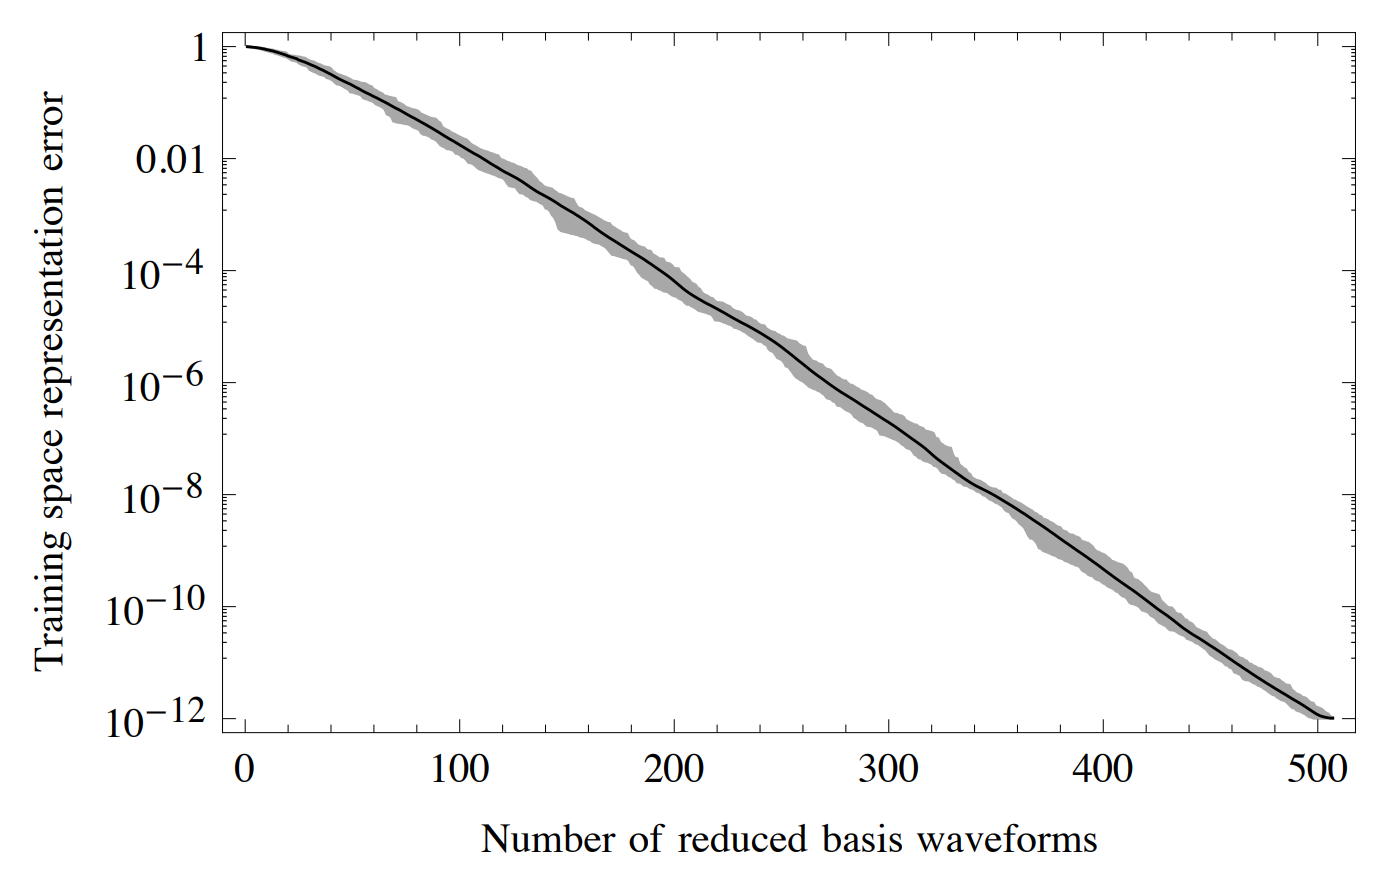
\includegraphics[width=.8\columnwidth]{figs/rb_vs_n.png}
\caption{Error de representación en función del número de funciones de onda en la base reducida para un modo cuasinormal (QNM). Se probaron todas las semillas posibles del conjunto de entrenamiento; en negrita se ve el promedio, y el área sombreada representa los valores extremos \cite{Caudill_2012}.}
\label{fig:rb_vs_n}
\end{figure}